\chapter{Introduction}
\section{Lithium ion battery (LIB)}
\subsection{The features of LIB\textsuperscript{[1]}}
Primary Li batteries were invented in the 1970s by M. Stanley Whittingham and then developed by John B. Goodenough and Akira Yoshino[1]. LIBs have been one of the most predominant power sources ever since 1991. Compared to other secondary batteries such as Nickel-Cadmium battery (NiCd), Nickel-metal battery (Ni-M), LiBs are featured with the highest energy density, higher operating voltages, limited self-discharging, long cycle life, lower maintenance requirements, and environmental friendliness. Also, it is well known that they do not suffer from ‘memory’ effects that plague other batteries. These matchless advantages make LIBs commonplace in secondary battery market. 
\begin{figure}[h]
\centering
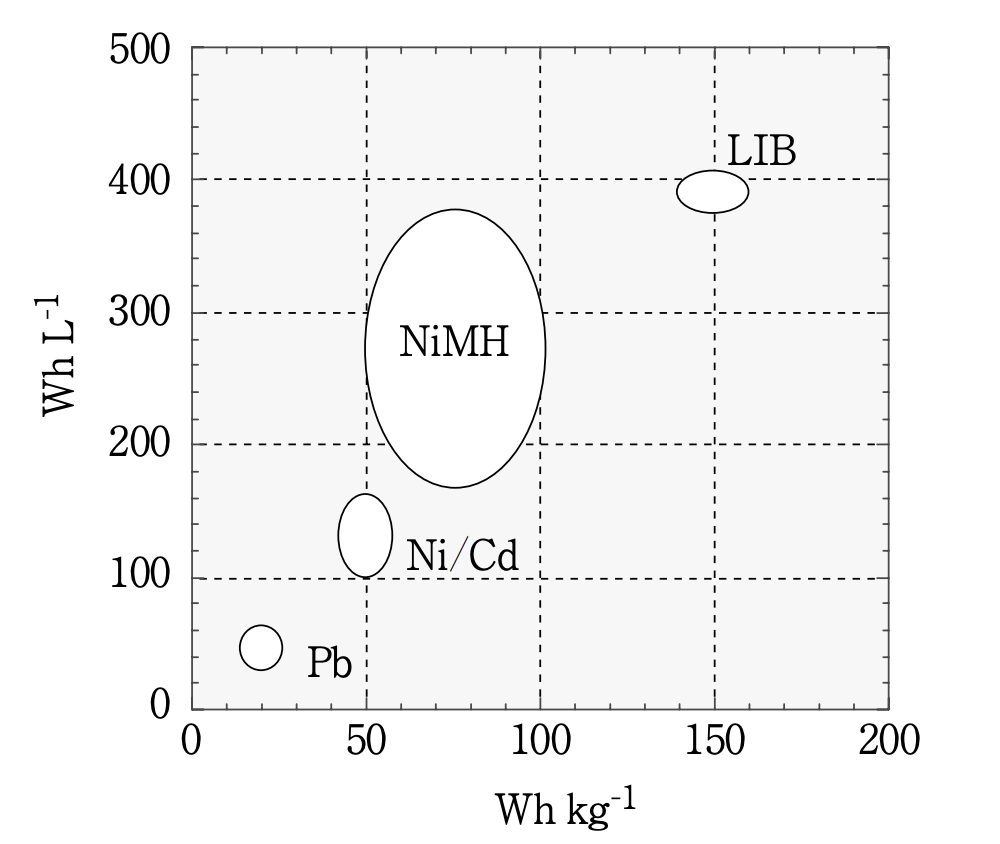
\includegraphics[width=8cm]{src/fig/fig1.png}
\caption{The energy density in different secondary batteries}
\end{figure}
However, for the practical applications in EVs where a large number of LiBs are packed together and used for high power output. The optimal performance LiBs is expected to be: (1)high specific capacity; (2)high durability and safe ; (3)long cycle life; (4)lightweight.

Since the current anode and cathode materials have almost reached their ideal capacities, the development of next-generation LiBs is expected through the research on new materials.

Generally, a lithium-ion battery consists of an anode, cathode, current collector, electrolyte, and separator. The electrodes repeat charging and discharging, converts chemical energy to electric energy, or vice versa, by redox reactions. Charging causes the Lithium ions within the crystal structure of the cathode material to be extracted and inserted into the anode material. During discharging, Lithium ions stored in the anode move to the cathode. The electrons travel through an external circuit thus forming a closed circuit. Both anodes and cathodes allow Li+ insertion and extraction without major changes to the host structure. A separator that allows ions to shuttle through, which is necessary to prevent from making direct contact between the electrodes.
\begin{figure}[h]
\centering
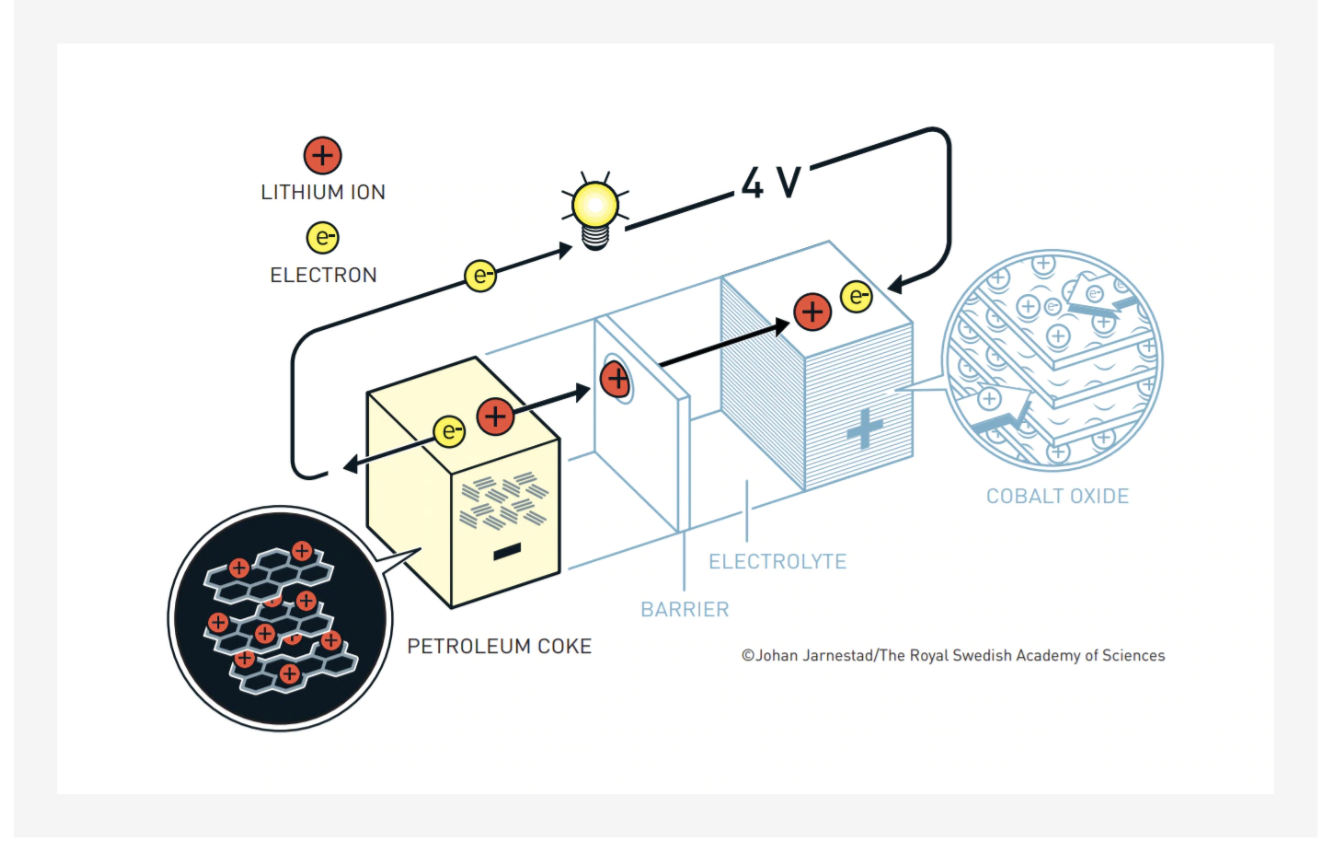
\includegraphics[width=8cm]{src/fig/fig2.png}
\caption{Schematic illusion of a LIB\textsuperscript{[2]}}
\end{figure}
The charging and discharging reactions of this battery can be expressed as follows:
$$L i_{1-x} C o O_{2}+x L i^{+}+x e^{-} \Leftrightarrow L i C o O_{2}$$
$$L i_{x} C_{6} \Leftrightarrow x L i^{+}+x e^{-}+C_{6}$$
\subsubsection{Cathode:}
The cathode, also called the positive electrode, functions within the battery as an oxidant during discharge. Cobalt-based cathodes ($\mathrm{LiCoO_{2}}$) are the most common cathode used in LiB due to high equilibrium potential. $\mathrm{LiCoO_{2}}$ has lithium and cobalt laminated between oxygen layers, and the charge/discharge reaction is repeated by intercalation–deintercalation of large amounts of lithium ions. In recent years, significant researchs have focused on other layered positive electrode materials, in which the Co or Ni of $\mathrm{LiCoO_{2}}$ and $\mathrm{LiNiO_{2}}$ are replaced by other transition metals. 
\subsubsection{Anode:}
The anode, as the negative electrode active material, is a reducing agent with a lower potential during discharging. So anode materials should have a low potential corresponding to a standard electrode and provide a high cell voltage with the cathode. Graphite-based anodes are the dominant materials in the anode market for their low voltage, excellent performance, and most of all, low cost. However, nowadays, the low capacity of graphite no longer meet the energy needs. Materials like Si and Sn have with higher capacity have attracted scientists attention.
\subsubsection{Electolyte:}
Within a battery, the electrolyte is the most important component after the positive and negative electrodes. For a practical battery, the choice of electrolyte often has a large effect on the characteristics of the battery, such as the operating voltage and the energy density. A wide variation of electrolytes has been used in solid, molten or liquid form.
The following gives some of the general properties that an electrolyte for a practical battery should have:
\begin{itemize}
\item High ion conductivity
\item Wide potential window
\item Thermal and chemical stability
\item No or low toxicity
\end{itemize}
The major discovery of electrolyte focus the selection of binary solvent mixtures such as ethylene carbonate (EC) and either dimethyl carbonate (DMC), ethyl methyl carbonate (EMC) or diethyl carbonate (DEC), and the Li salt, lithium hexafluorophosphate ($\mathrm{LiPF_{6}}$), as the basic standard electrolyte solutions for Li-ion batteries.
\subsubsection{Separator:}
Separators are nonactive materials that do not participate in electrochemical reactions. They provide a pathway for ion transport that is essential for battery operation and separate physical contact between the anode and the cathode. Typically, separators are micro porous polymer films with a porosity of 30–50\% and the thickness ranging from manometers to micrometers. The most commonly used separators are polyolefins such as polyethylene(PE) and polypropylene (PP), and these materials have various advantages including outstanding mechanical strength, chemical stability, and low cost. If the temperature rises during internal short circuits, the melted separator blocks pores and restricts ion movement, thus improving battery safety by delaying thermal reactions.
\subsubsection{Cell container:}
The components of LIB should  be appropriately packaged in a container. To satisfy the requirement of lightweight and robust, metal containers are often used. In addition, thermal exchange properties and crush/crash worthiness are also important factors for a long-term service of battery. Rubber gaskets used in a container act as seals to prevent electrolyte from leaking out and moisture in the air from infiltrating the battery.
\subsection{Next-generation Si-based anodes\textsuperscript{[1]}}
Graphite is the most commonly employed material in the LIB anode due to its low cost and good stability. Graphite is composed of hexagonally bonded sheets of $\mathrm{sp^{2}}$ hybridized carbon that bounds with sub-sequent sheets through van der Waals force. Intercalation/deintercalation process (the insertion/withdrawal of Li+ ions) takes place in between the planes of the graphite. The formation of intercalation compound $\mathrm{LiC_{6}}$ provides a theoretical specific capacity limit of 372 mAh/g.
To satisfy the need for large-scale portable energy sources, alloy-type anodes have been intensively explored due to their high capacity. From a material’s point of view, Silicon(Si) has been receiving tremendous attention in recent years. First, the discharging potential of Si, about 0.2 V with respect to Li/Li+ , is lower than most of other alloy-type or metal oxide anodes. Second, Silicon has the highest theoretical capacity of 4200 mAh/g upon full lithiation with the formation of $\mathrm{Li_{22}Si_{5}}$, which is more than 10 times that of commercial graphite. Third, there is a high abundance of Si element in the earth crust and the cost to obtain both single-crystalline and polycrystalline Si has dropped to an acceptive range. Also, there are other merits of Si, such as good environmental compatibility, low toxicity, and relatively stable chemical compatibility, low toxicity, and relatively stable chemical property, and all these make Si a very promising candidate for next-generation anode.
\begin{figure}[h]
\centering
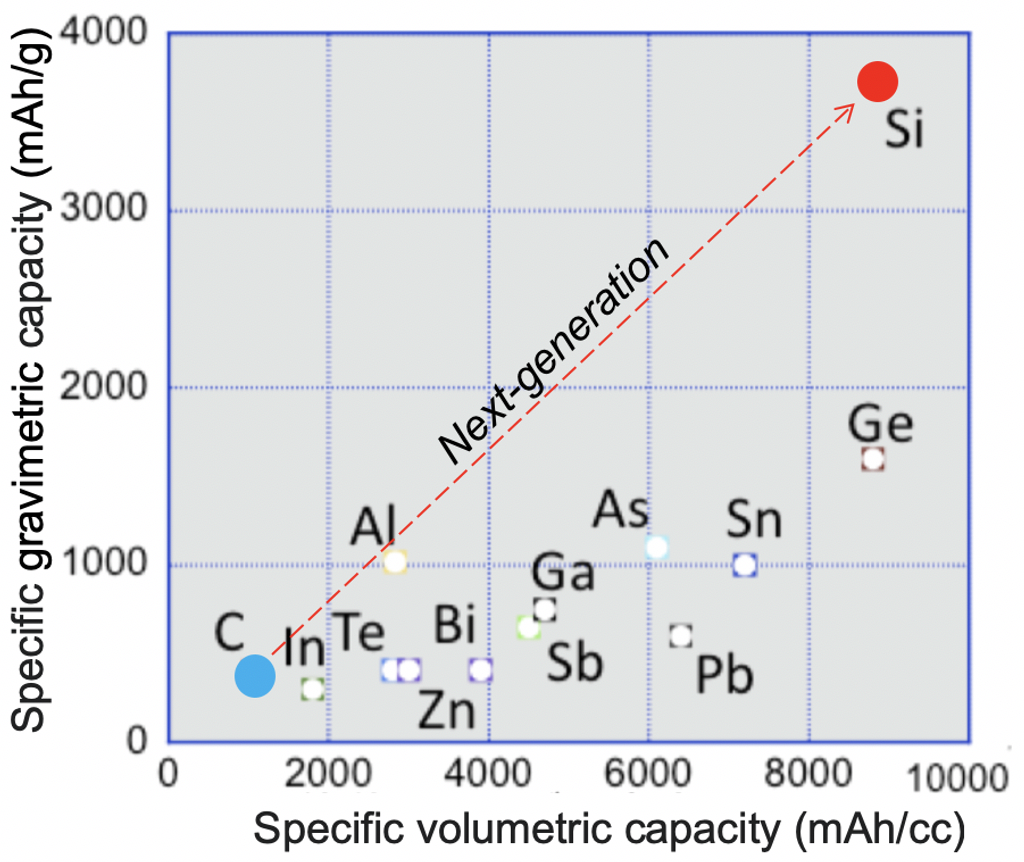
\includegraphics[width=8cm]{src/fig/fig3.png}
\caption{The specific capacity of elements}
\end{figure}
However, the practical implementation of Si anodes is still blocked due to three major problems. First, silicon has poor electronic conductivity. Second, Si anode usually suffers from large volume change (>300\%) and mechanical fracture within 10 cycles. Finally, the solid electrolyte interphase (SEI) breaks as the nanostructure shrinks during delithiation. This results in the exposure of the fresh silicon surface to the electrolyte and the reformation of the SEI, resulting in the SEI growing thicker with each charge/discharge cycle. These side effects lead to poor cycle-life, drastic irreversible capacity loss and low coulombic efficiency of Si anode. other high capacity materials such as tin (Sn), germanium (Ge), and antimony (Sb) have the same volume change issue. 

To address these issues, several strategies have been developed to accommodate the huge volumetric changes. Tremendous exploration on materials has been made.
\begin{figure}[H]
\centering
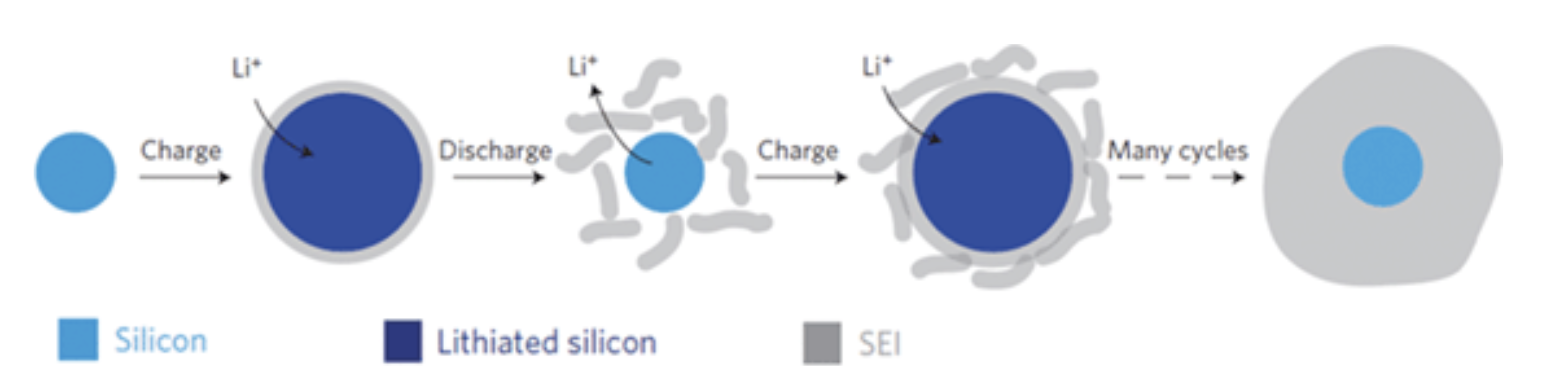
\includegraphics[width=10cm]{src/fig/fig4.png}
\caption{Schematic of SEI formation on silicon surfaces\textsuperscript{[3]}}
\end{figure}
As one effective strategy to suppress the volume change, Silicon is produced in dimensions of tens of nanometers. According to the research of J. Graetz\textsuperscript{[4]}, nanocrystalline silicon exhibited specific capacities of ~ 1100 mAh/g with a 50\% capacity retention after 50 cycles. The amorphous thin-film electrodes exhibited initial capacities of 3500 mAh/g with a stable capacity of ~2000 mAh/g over 50 cycles. The capacity and cycle performance were greatly enhanced in nano-size Si structure, compared with bulk Si.
\begin{figure}[H]
\centering
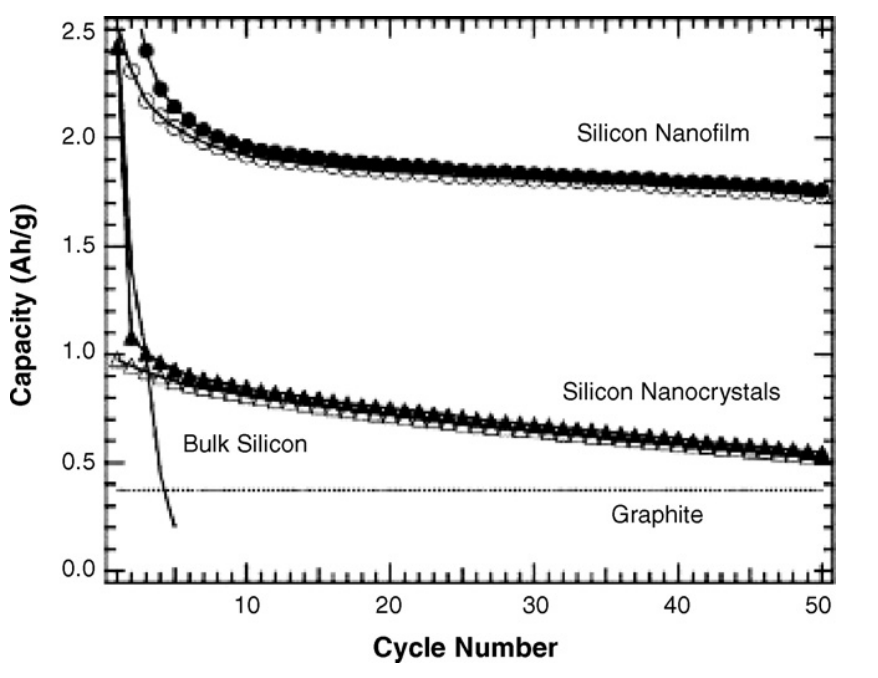
\includegraphics[width=8cm]{src/fig/fig5.png}
\caption{Specific capacity vs. cycle number for nano-crystalline Si, nano-amorphous Si thin film anodes, graphite and bulk-silicon anodes\textsuperscript{[4]}}
\end{figure}
\begin{figure}[H]
\centering
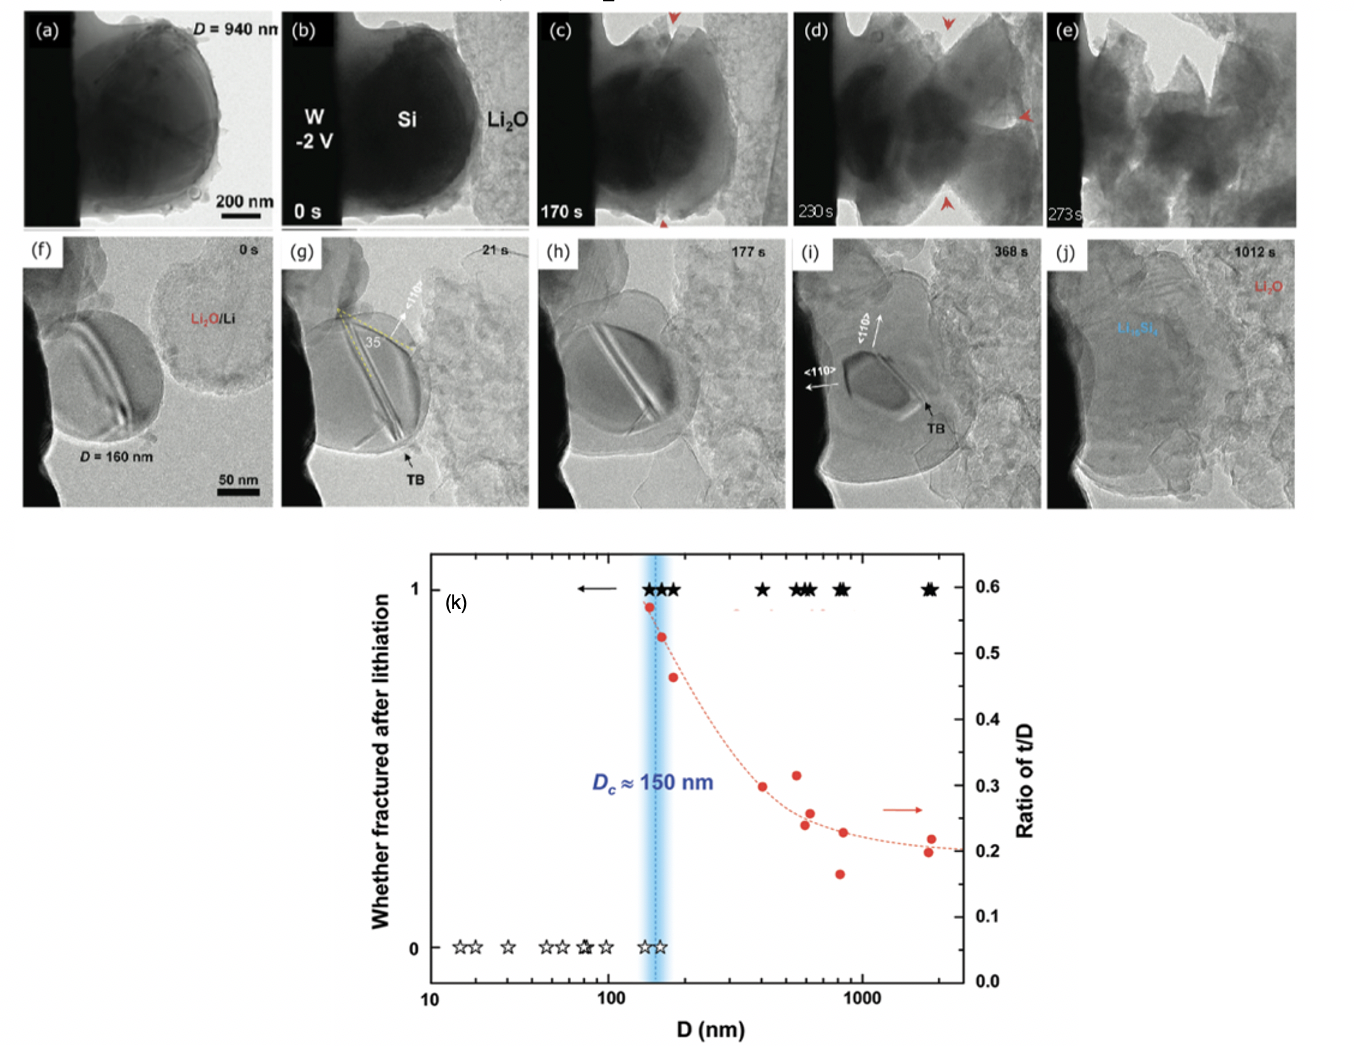
\includegraphics[width=14cm]{src/fig/fig6.png}
\caption{The lithiation of SiNP with diameter (a)--(e) D=940 nm, (f)--(j) D=160 nm, (k) The relationship between Si particle size and fracture.\textsuperscript{[5]}}
\end{figure}
The in situ TEM observations by Liu\textsuperscript{[5]} confirmed that the lithiated Si structure breaks during Li alloying reaction process in one minute. As shown in figure 1.6, the pristine SiNP (D=940 nm) multiple cracked at different locations eventually fracture occurred. In contrast, for a smaller SiNP (D=160 nm), no cracks was observed till Si attained full lithiated state $\mathrm{Li_{15}S_{4}}$. This observation was in good agreement with critical size $\mathrm{D_{C}}$ of about 150 nm, which was from statistics result. 
In addition, figure 1.6(i) shows the expansion along <110> directions is 170\%, while along <111> directions the swelling is less than 20\%. This result indicates that lithiation-induced swelling is preferably along the <110> directions in Si nanowires, which is consistent with the anisotropic expansion of the SiNP.

Despite the advantages of nanostructured Si anodes, nanosized particles also have disadvantages such as large surface area, high manufacturing costs, and difficulty of handling. Even so, nanostructured silicon is regarded as one of the most promising methods to overcome the challenges of silicon anodes for next-generation lithium-ion batteries.
%\vspace{-10em}
\subsection{Si@carbon nanocomposite}%1.1.3
%\vspace{-7em}
Another approach to overcome the volume change during cycling is to form Si-carbon composites. The carbon material is usually used ad a buffer matrix that prevents the significant volumetric change of Si, maintaining the structural integrity of the electrode, and enhancing stability by reducing silicon aggregation or electrochemical sintering. Also, due to the limited electrical conductivity of Silicon, carbon additives can improve battery performance. There are several structure designs of Si-carbon composite.
%\vspace{-14em}
\subsubsection{(i)core-shell/yolk-shell\textsuperscript{[6]} }
%\vspace{-7em}
\begin{figure}[H]
\centering
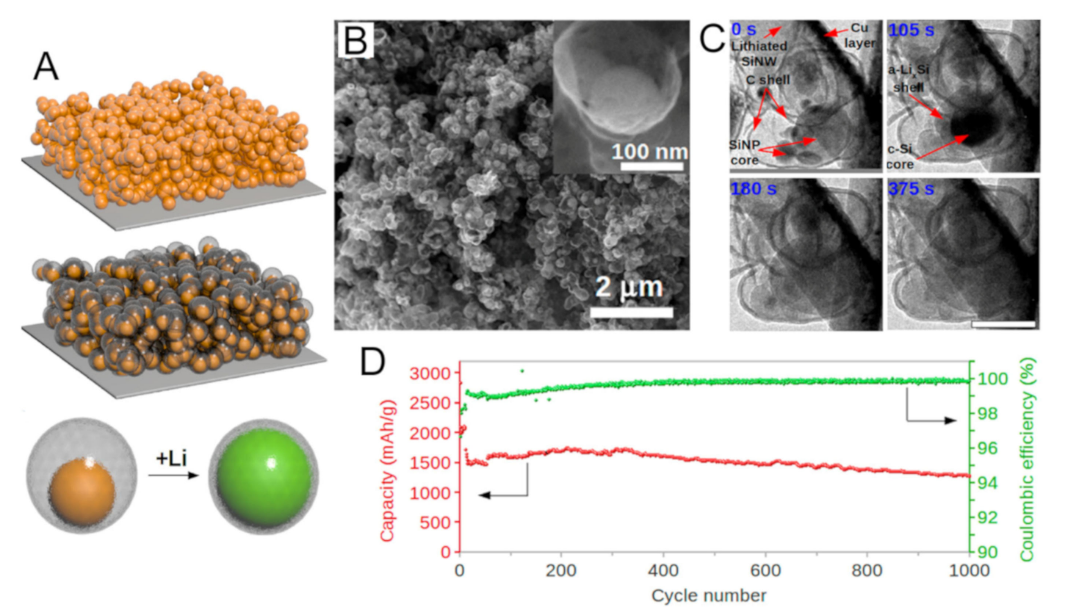
\includegraphics[width=14cm]{src/fig/fig7.png}
\caption{Si@C yolk–shell nanostructure. (A) Comparison of a conventional slurry coated SiNP and Si@C yolk–shell nanostructure. (B) SEM image of Si@C yolk–shell nanostructure. (C) Serial in situ TEM images showing the expansion of the Si yolk part. The scale bar is 200 nm. (D) Delithiation capacity and Coulomb efficiency of the first 1000 galvanostatic cycles between 0.01-1 V at 1 C rate.\textsuperscript{[6]} }
\end{figure}
Core-shell/yolk-shell nanostructures indicate a class of hybrid materials consisting of a hollow shell encircling movable cores with the void. The additional space between the core and the shell, usually carbon or silicon oxide, can buffer the volume expansion significantly. The outer shell remains unchanged during cycling, and thereby helps the formation of a stable SEI layer, thus electronic conductivity is promoted.
Cui and co-workers have made pioneer work in this field[4]. The completely sealed Si@C yolk–shell structure was monitored with in-situ TEM to demonstrate that the Si@C yolk–shell provides excellent electrochemical cycling performance to alleviate the severe volume change of Si during lithiation/delithiation (Figure 1-7C). Pristine Si nanoparticles (0s) are visible within the outer Carbon shell. The volume expansion of Si nanoparticles is seen in 105s to produce the partially lithiated LixSi shell/crystalline Si core in the carbon shell. Full lithiation increases the size of Si particles up to ~300 nm. Furthermore, the thickness of carbon shell increases from 5 to ~20 nm after lithiation implying that the carbon coating is also lithiated and creates a thin layer of ionic liquid electrolyte at the surface. Figure 1-7D shows the reversible capacity of Si@C yolk–shell electrode reached 2833 mAh/g for the initial cycle at C/10 and stabilized at ~1500 mAh/g at 1 C. No capacity retention was observed in the first 300 cycles and 74\% of the capacity was achieved after 1000 cycles. 
\subsubsection{(ii)Si-graphene/Si-carbon coating\textsuperscript{[7]}}
Graphene has also been used in Si anodes to buffer the volume changes and improve electronic conductivities due to its superior electrical conductivity, high surface area, excellent chemical stability, and strong mechanical strength. Pan[5] prepared silicon@carbon@graphene micro-sized composite (Si@C@RGO) using an industrially scalable spray drying approach and a subsequent calcination process. As fig.1-9 shows, The obtained Si@C@RGO anode exhibits a high initial reversible specific capacity of 1599 mAh/g at a current density of 100 mA/g. Moreover, the Si@C@RGO anode shows a high reversible specific capacity of 951 mAh/g  even at a high current density of 2000 mA/g . The excellent cycling stability and superior rate capability are attributed to the unique structural design of carbon coating and wrapped by highly conductive graphene. The combination of carbon shells and flexible graphene can effectively enhance the electrical conductivity of the composite and accommodate significant volume changes of silicon during cycling.
\begin{figure}[H]%  强制放图片
\centering
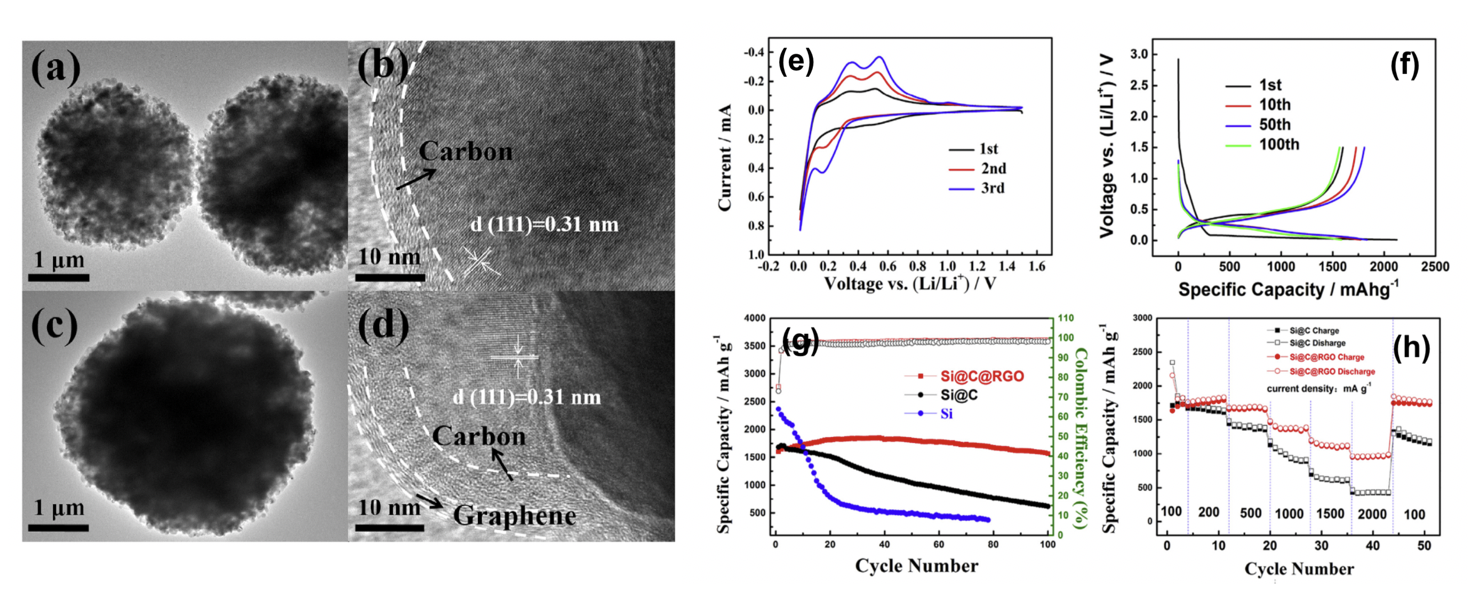
\includegraphics[width=14cm]{src/fig/fig8.png}
\caption{HRTEM images of (a, b) Si@C and (c, d) Si@C@RGO
composite;(e) CV curves of the Si@C@RGO anode at 0.1 mV/s  between 0 and 1.5 V for the first three cycles; (f) Charge/discharge voltage profiles of Si@C@RGO composite for the 1\textsuperscript{st}, 10\textsuperscript{th}, 50\textsuperscript{th}, 100\textsuperscript{th} cycle; (g) Cyclic performance of Si, Si@C and Si@C@RGO composite at a current density of 100 mA/g in the first three cycles and then continued at 200 mA/g thereafter; (h) Rate performance of Si@C and Si@C@RGO composite at various current densities\textsuperscript{[7]}.}
\end{figure}

\subsubsection{(iii)Si-carbon nanotubes(Si@CNF)/Si-carbon nanofibres(Si@CNF) composite\textsuperscript{[8]}}
Recently, CNTs has received considerable attentions as a candidate material for the LIB application. Different from other allotropes of carbon, CNT is a 1D structure with a large aspect ratio(length--to--diameter) in excess of 1,000. CNTs can be regarded as nanoscaled cylinders composed of rolled up graphene sheets around a central hollow core. There are two types of CNTs: single-walled carbon nanotubes (SWCNTs) and multi-walled carbon nanotubes (MWCNTs), and the later consist of two or more graphene layers with van der Waals forces between adjacent layers. However, growing  SWCNTs requires strict growing condition such as high temperature. That is because their small diameters results in high curvature and high strain energy to maintain its crystalline. A perfectly structured CNTs possess amazing mechanical properties such as Young’s modulus, which are favored especially in energy storage field. This is due to the chemical bonding of $sp^{2}$ in CNTs. 

As to application of CNTs in LIB,the incorporation of CNTs as an additive to active materials is an effective strategy to form conductive networks in the electrode at a content much lower than other carbonaceous materials, like carbon black and graphite. Various anode materials with and without CNT additives have been studied, undeniably confirming much enhanced cycle performance of the nanocomposites containing MWCNTs as compared to the neat anode materials.

MARUBAYASHI\textsuperscript{[9]} had employed the thin-layered graphite (TLG) and the artificial graphite (AG) as conductive additives for improving the conductivity of the $\mathrm{LiCoO_{2}}$ (LCO) cathode, in either case the small amount of MWCNT improved the capacity retention ratio. Xue et al.\textsuperscript{[10]} had produced carbon coated Si nanoparticles then dispersed them in a CNT network. Electrochemical test result indicates the Si@C-CNTs show capacity retention of 70\% after 40 cycles, which is much better than the Si@C nanoparticles without CNTs. The tangled CNT network is believed to  better accommodate of the strains arising from Li ion insertion/extraction to maintain the integrity of electrodes, stabilize the electric conductive network for active Si, and eventually lead to better cycling performance. In addition, it is reported that The CNTs can facilitate rapid Li ion transport through the large electrode–electrolyte contact area and work as fast electron transport pathways.[6] 
\begin{figure}[H]
%\centering
\begin{minipage}[t]{0.5\textwidth}
 \centering
 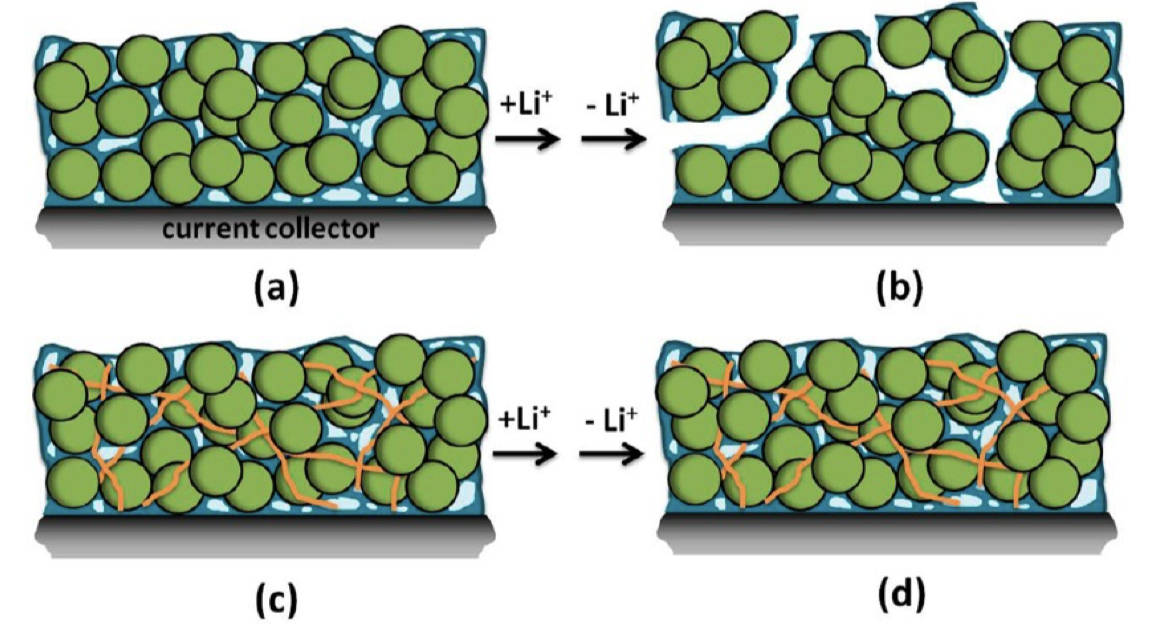
\includegraphics[scale=0.35]{src/fig/fig9.png}
 \caption{Schematic of a Si@C with binder (a) before and (b) after cycling, and Si@C--CNTs with binder (c) before and (d) after cycling\textsuperscript{[10]}.}
 \end{minipage}
%\hfill
\begin{minipage}[t]{0.5\textwidth}
%\centering
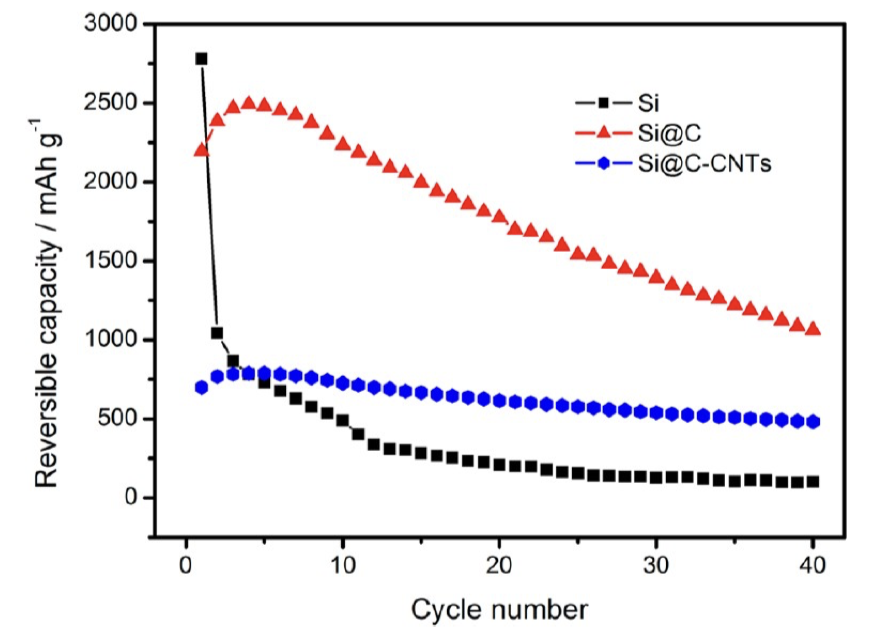
\includegraphics[width=7cm]{src/fig/fig10.png}
\caption{Cycling performance of Si, Si@C, and Si@C-CNTs at 100 mA\/g and within a voltage window of 0.02-2.0 V\textsuperscript{[10]}.}
\end{minipage}
\end{figure}

The term  ‘tube’  refers to those sheets rolled up into concentric cylinders. If the stacked-cone structures exhibit only small $\theta$  values and are not cylinders but are mostly hollow, the can be called multi-walled carbon nanofibres (MWCNFs). Also, CNFs are much bigger,more disordered, less oriented, with a large number of  defects.  Hence the mechanical properties of CNFs are as  outstanding as of CNTs, especially the single-walled ones , but still high enough to be used in LIB. [Effect of CVD carbon coatings on Si@CNF composite as anode for lithium-ion batteries]). On the other hand, defective CNTs were reported to be more effective for the adsorption and diffusion of lithium ions. 

\section{Plasma-spray PVD}
\subsection{Feature of plasma\textsuperscript{[11]}}
Plasma is the fourth state alongside solids, liquids, and gases. It is a special kind of ionized gas and in general consists of positively charged ions , electrons, and neutrals (atoms, molecules, radicals). A typical example is the sun, whose interior temperatures exceed 107K. The plasma stays quasi-neutral and its properties are dominated by electric and/or magnetic forces .
There are two types of plasma, non-thermal plasma and thermal plasma. Non-thermal plasma is usually generated by glow discharge at low pressure, and mostly contains unionized neutral gas particles. In a non-thermal plasma, only the electron temperature($T_{e}$) is high and other species like heavy particles and ions stay at relatively temperature. Therefore, such plasma is called non-equilibrium plasma or low temperature plasma as well. On the other hand, thermal plasma is generated by arc discharge at higher pressure range, which possess a higher ionization level. The electron temperature Te, ion temperature Ti, and neutral temperature Tn are almost equal (5,000 K -- 20,000 K).

\begin{figure}[h]
\centering
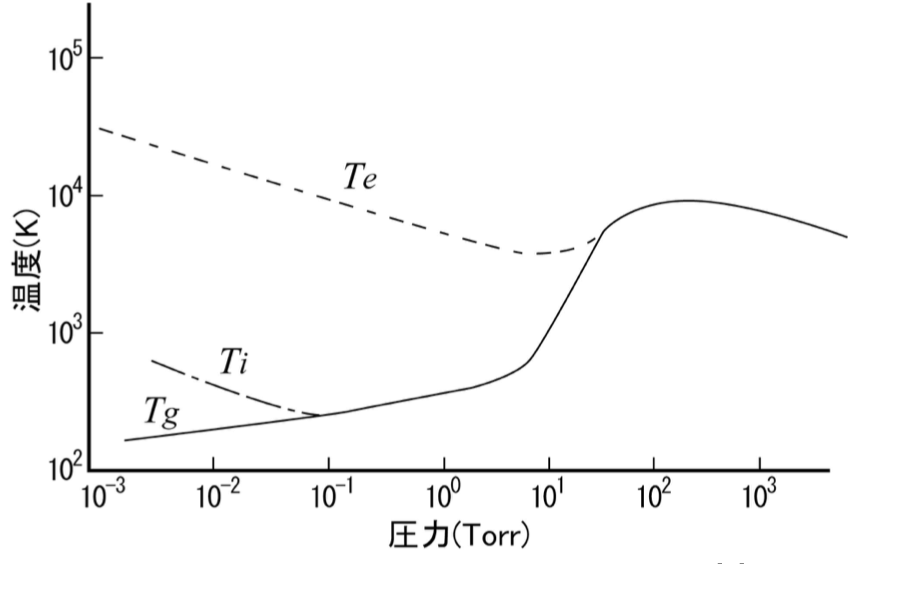
\includegraphics[width=8cm]{src/fig/fig11.png}
\caption{The temperature in a plasma as a function of pressure\textsuperscript{[14]}}
\end{figure}
Today, plasma technology is applied to the field of deposition of coatings and films. One typical method is Plasma spray physical vapor deposition (PS-PVD). PS-PVD is recognized as a high throughput process for production of nanoparticles and nonstructural coatings by completely evaporation, quenching and condensation on a relatively cooler substrate. Compared to other surface coating technologies, the major advantages of PS-PVD are as follows:
\begin{itemize}
  \item The thermal plasma can heat up feed stock materials quickly and effectively, for its high temperature and active species. Therefore, the deposition rate is high, enables PS-PVD technology to meet the industrial requirements.
  \item The substrate can stay at a relatively low temperature, namely the quality of the substrate itself can be maintained.
  \item By selecting different gases to generate plasma, it is possible to create a wide range of conditions, such as oxidizing atmosphere ($\mathrm{O_{2}}$), inert atmosphere (Ar), or reducing atmosphere ($\mathrm{H_{2}}$), etc.
\end{itemize}

\subsection{Types of Plasma spray\textsuperscript{[15]}}
Plasma spraying systems can be categorized into three types based on the plasma jet generation method.
\begin{figure}[H]
\centering
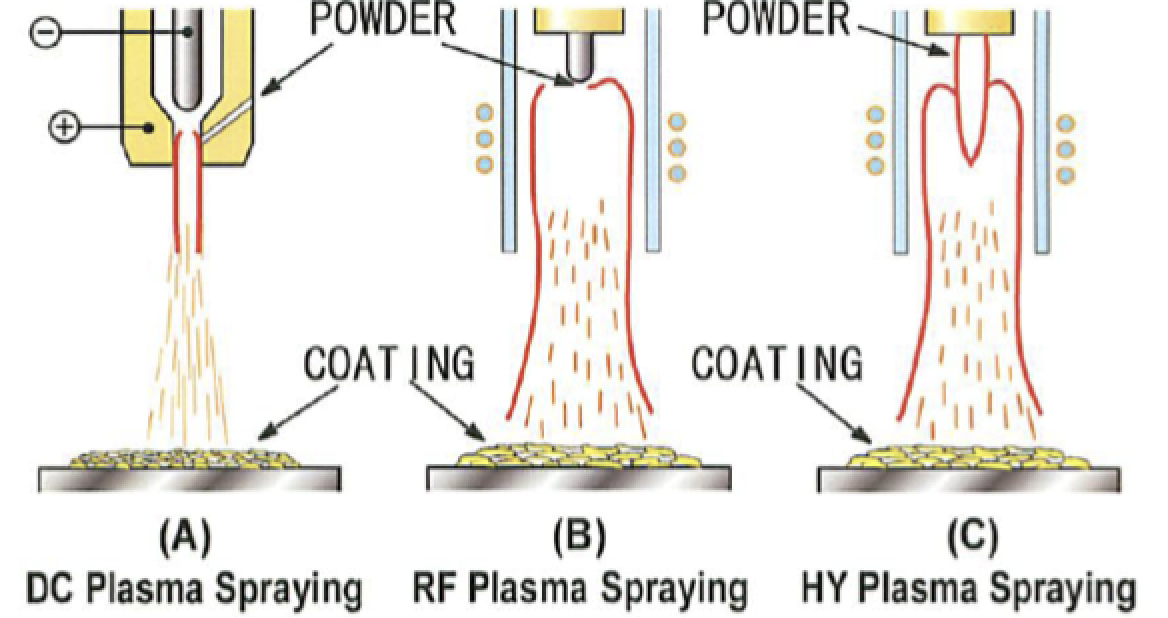
\includegraphics[width=10cm]{src/fig/fig12.png}
\caption{Plasma generated by (a)direct current; (b)radio frequency; (c)hybrid torch\textsuperscript{[15]}}
\end{figure}
\subsubsection{(a)	Direct-current (DC)}
A high--intensity arc is generated by a direct current and operated between a stick-type cathode and a nozzle-shaped anode. This Cupper anode is usually water-cooled, establishing a sharp temperature drop in plasma, in order to confine the arc expansion and guarantee an energy constriction. This effect is called “thermal pinch”. The figure below shows the temperature and flow velocity distribution of a typical Ar-$\mathrm{H_{2}}$ DC plasma. It is generated at an arc voltage of 52V, an arc current of 500 A. The flow rate of Ar is 44 L/min and of $\mathrm{H_{2}}$ is 7 L/min. There is a sharp temperature and velocity drop along with the axial directions. Using the enthal--peeve method, the temperature gradient is found to be 250 K/mm and the velocity gradient is about 10 m/s/mm. Ideally, the powder should be fed to the center of the plasma for sufficiently evaporation. However, but in DC plasma, the powder is injected in the direction that is perpendicular or angled(45°) to the plasma jet. The plasma gas is highly viscous and flows at high speed, the lightweight particles and heavy particles are carried at different orbits, result in an nonuniform coating.
\begin{figure}[H]
\centering
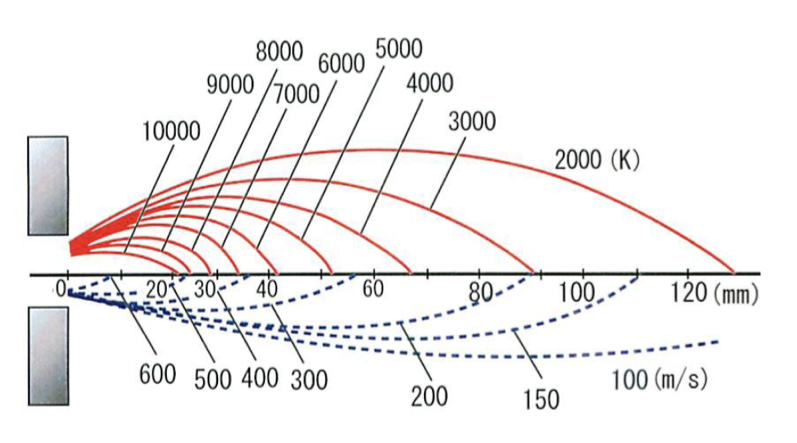
\includegraphics[width=10cm]{src/fig/fig13.png}
\caption{The temperature and velocity axial distribution in DC plasma jet\textsuperscript{[13]}.}
\end{figure}

\subsubsection{(b) Radio-frequency (RF)}
There are several types of plasma that use radio frequencies, but here the most used one, inductively coupled plasma (ICP), is addressed. In ICP, The current produced by electromagnetic induction, namely, by time-varying magnetic fields. This current flows in a cylindrical coil that surrounds the plasma bulk. The frequency for generating plasma is determined by the diameter, gas type, and power. The benefits of using ICP are as follows:
\begin{itemize}
  \item Due to the absence of electrodes in an ICP, the axial injection of the feed stock is realised.
  \item The RF discharge permits particles a relatively long in-flight heating time and low velocity(20--30 m/s), which is about an order of magnitude lower than that of DC plasma. As a result, the residence time of substances in the plasma is about 10 ms, and the particles can be melted uniformly and sufficiently.
  \item It is possible to generate plasma that cannot be obtained by other methods such as $\mathrm{O_{2},Cl_{2}, and  F_{2}}$, and there is no contamination of impurities by the electrode material.
  \item A large volume plasma with a diameter of several centimeters can be easily obtained. This is equivalent to 10 times that of a DC plasma.
\end{itemize}
Nevertheless, there are still some cons of ICP. Since the particle velocity is slow, for some materials with high melting point, it's difficult to form a dense film because the droplets already condense before arriving to the substrate. In addition, Since ICP is an electrode--less discharge, the eddy current generated at the time of injecting feed stock is inevitable and cause disturbance to the stability of plasma.

\subsubsection{(c) RF-DC hybrid plasma}
A hybrid plasma is a developed method that combines DC and RF discharge. In hybrid plasma, the DC arc jet is superimposed on the RF plasma centrally, eliminate the possibility of the eddy current generation. In RF, the flow velocity could hardly be controlled, but in hybrid plasma, the input powder rate can be controlled by changing the input of DC plasma, and the appropriate in-flight heating time. Therefore, even for in high melting point materials, the time for staying in the droplet state can be extended till arriving at the substrate, thus a dense film is formed. In hybrid plasma, the temperature distribution is more uniform than that in RF plasma, as shows in fig 1.14.
\begin{figure}[h]
\centering
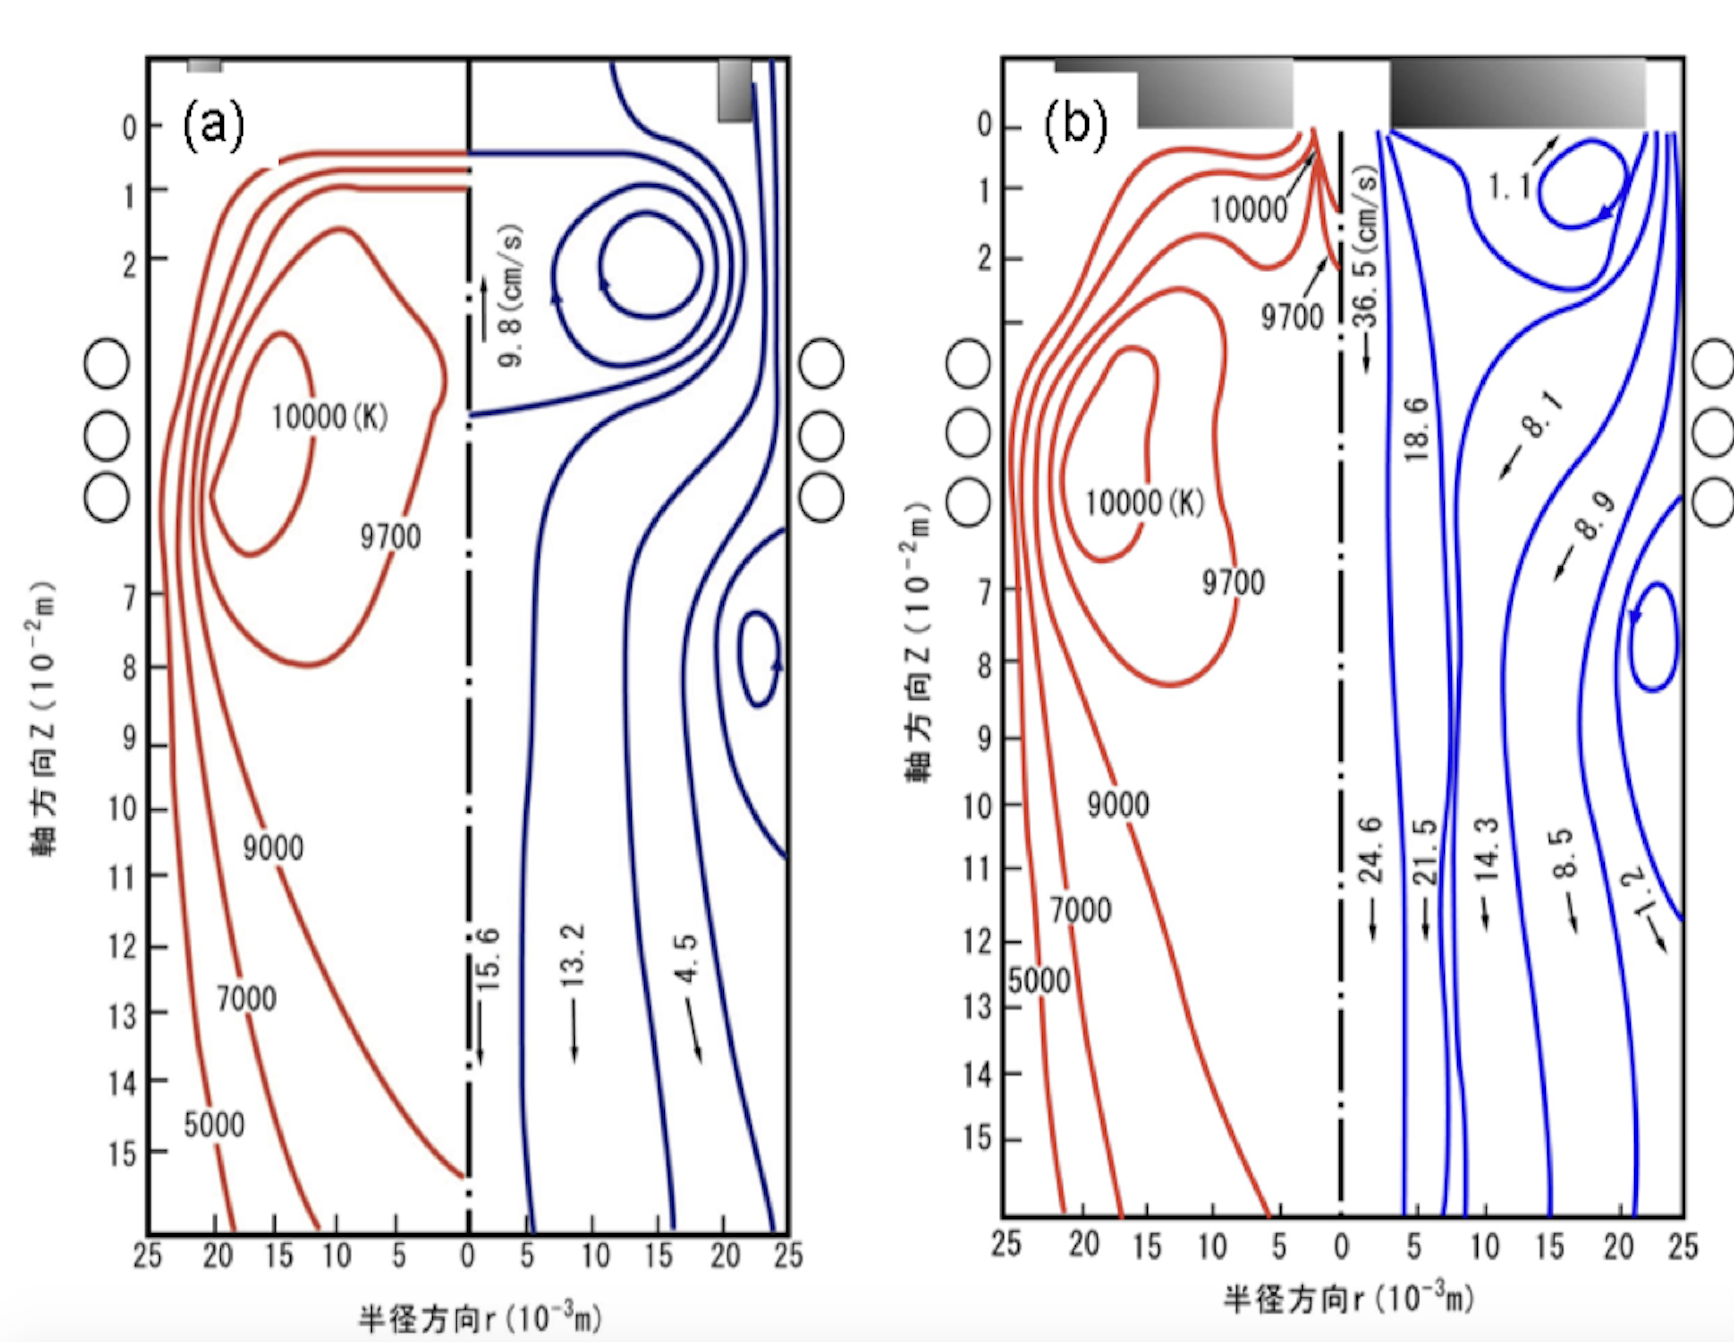
\includegraphics[width=8cm]{src/fig/fig14.png}
\caption{The temperature and velocity distribution in (a) RF plasma (b)Hybrid plasma\textsuperscript{[16]}}
\end{figure}
%没有别的介绍了吗? 我怎么知道你要用PS-PVD去做纳米粒子???
\section{Plasma Enhanced-CVD}
As an advanced method to grow carbon nanotubes, plasma-enhanced CVD features with its low-temperature. In general, carbon nanotubes are produced by basically three methods: laser furnace, the arc, and chemical vapor deposition (CVD). Laser methods are not for large-scale production. The problem with arc material is purification. Thermal CVD and Plasma-enhanced CVD are the popular methods among the market for their salable production, the former method usually requires growth temperature over 700\(^\circ\)C, which is unfavorable for electronic device production. Thus plasma is introduced to lower the temperature of CNT growth. In plasma-enhanced processes, the plasma creates many new and a larger number of reactive species, such as radicals, ions and molecules in excited states, and thus enhances adsorption of carbon-bearing molecules on the catalyst particles providing higher growth rates of the structures as compared with thermal CVD. 

\subsection{Glow discharge\textsuperscript{[16]}}
Typically a glow discharge at reduced pressure is favored for the CNT growth.  As shown in fig.1-15, a glow discharge should be non-thermal, that is, the electron temperature is high but temperature for the heavy species is low.  There are various types of glow discharge plasma. 
\begin{figure}[h]
\centering
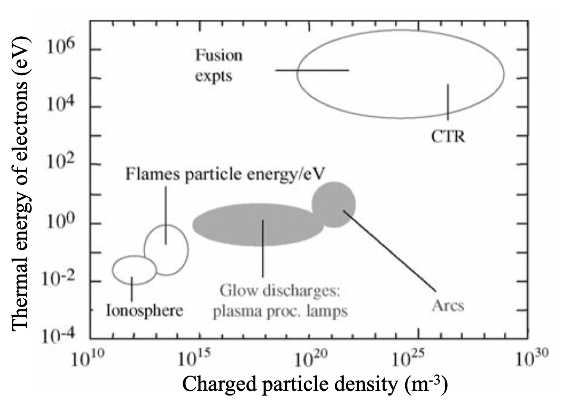
\includegraphics[width=8cm]{src/fig/fig15.png}
\caption{The particle density and electron energy of different plasma\textsuperscript{[16]}.}
\end{figure}
According to Townsend discharge theory, the ignition of plasma needs the electrical breakdown of a gas. The extracted free electrons are accelerated by an electric field, collide with gas molecules, and consequently free additional electrons. Those electrons are in turn accelerated and free additional electrons. The basic version is the direct current (DC) glow discharge, where a continuous potential difference is applied between the fixed cathode and anode, producing a constant current. The breakdown voltage for a specific gas in vacuum is a function of the product of  pressure and distance, which is given by Paschen. 
\begin{figure}[h]
%\centering
\begin{minipage}[t]{0.5\textwidth}
\centering
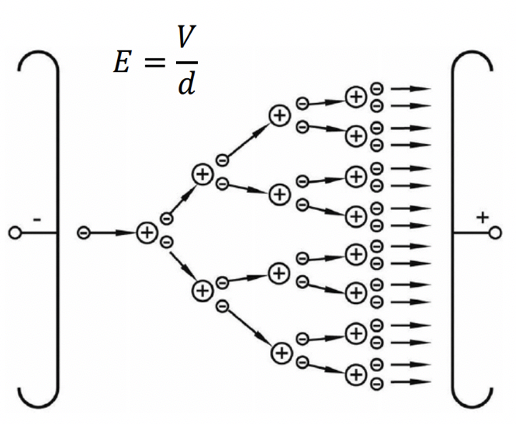
\includegraphics[width=6cm]{src/fig/fig16.png}
\caption{Townsend electron avalanche}
\end{minipage}
\hfill
\begin{minipage}[t]{0.5\textwidth}
%\centering
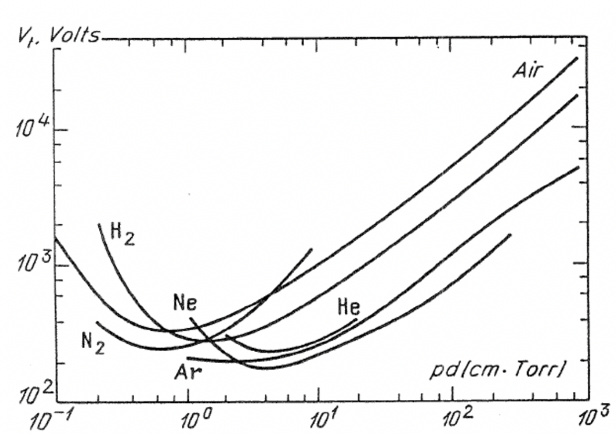
\includegraphics[width=7cm]{src/fig/fig17.png}
\caption{Typical Paschen’s curves\textsuperscript{[17]}}
\end{minipage}
\end{figure}
However, DC glow discharge may give rise to problems when one of the electrodes is non$-$conducting, as due to the constant current, the electrodes will be charged up and leading to burn-out of the glow discharge.  RF breakdown is similar to DC case except that the  high$-$confines electrons by field oscillations$-$multiplication replenishes diffusive losses. Thus the electrons are not as mobile as in DC case.  
\subsection{Low$-$temperature CNT Growth\textsuperscript{[19]}}
Researchers have investigated into growth mechanism of CNT for years. The pioneering work is made by Baker\textsuperscript{[18]}. Researchers have reported various mechanisms. The growth mechanism for most cases proceed as following: (i) the carbonaceous precursors are decomposed onto catalyst and (ii) the atomic carbons diffuse and form a graphitic tubular structure around the particles to form a nucleation seed. (iii) CNT growing from nucleation seed.  It is noteworthy that it’s still unclear whether carbon atoms diffuse on the particle bulk on the particle surface or whether surface and bulk diffusion compete.  

Typical hydrocarbon sources used in plasma-based growth of CNTs include methane, ethylene and acetylene. Since plasma can dissociate the hydrocarbon creating a lot of reactive radicals, the use of pure hydrocarbon feed stock may lead to substantial amorphous carbon deposition, which terminates CNT growth earlier. Therefore, it is desirable to dilute the hydrocarbon with argon, hydrogen or ammonia\textsuperscript{[20]}.
Transition metal catalysts are needed for CNT growth by PECVD, usually Ni, Fe,Co and Mo. Note that the catalyst should be in the form of particles as small as possible in the nanometer range\textsuperscript{[20]}.
\begin{figure}[H]
\centering
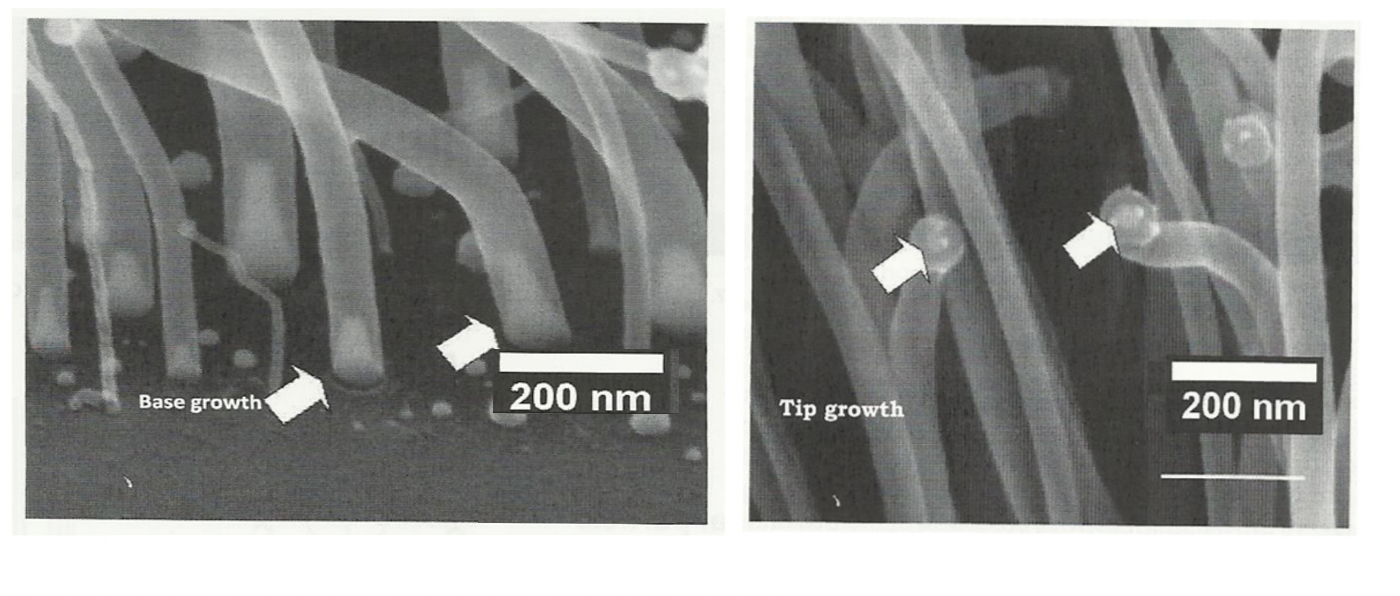
\includegraphics[width=10cm]{src/fig/fig18.png}
\caption{SEM image reveals (a) the base ends of CNTs (b) metallic particles located at the tip of CNTs\textsuperscript{[21]}}
\end{figure}

As fig.1-18 shows, there are two principal morphology of CNT.  The metal catalyst if enwrapped in CNT either within the root or  head. The former is called “base growth”, which usually occurs when metallic particle has strong enough interaction with substrate that cannot be easily separated by the graphite layer formed at the interface in between. On the other hand, if metallic particle and substrate are not strongly connected, the particles will detach and move towards the head of growing nanotubes. This labeled as “tip growth”. 

Generally, according to the state of metal catalyst, the mechanisms can be classified into vapor-solid-solid (VSS), vapor-liquid-solid (VLS) mechanism. V refers to the vapor that contains carbon source.  The middle term  refers to the state of metal catalyst, liquid or solid, dependent on the temperature.  The last term means the solid CNT. In VSS model, to keep the metal catalyst in its solid state, typically a low-temperature condition is needed. Especially in our research,  the solid state of metal catalyst (in our case, Nickel) is of great interest, for the purpose of suppressing silicidation since there is no diffusion barrier. 
\begin{figure}[H]
\centering
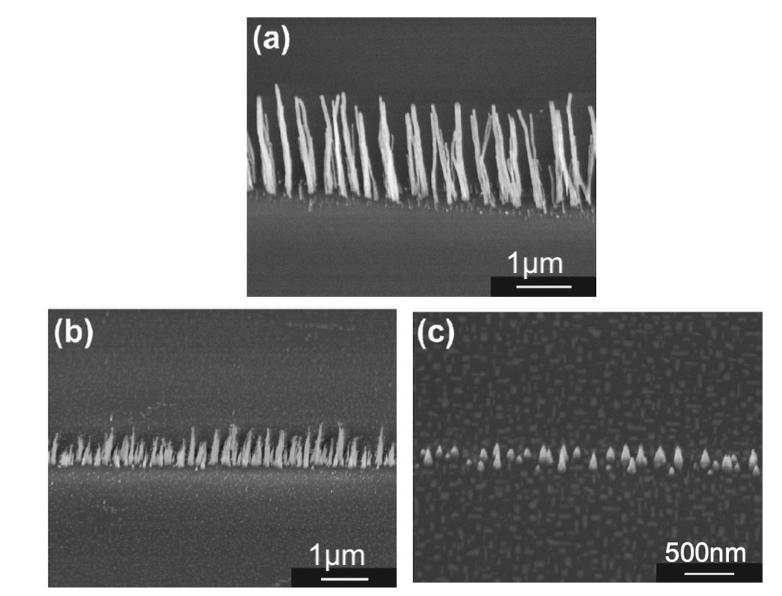
\includegraphics[width=10cm]{src/fig/fig19.png}
\caption{SEM photographs of vertically aligned CNFs grown from e-beam patterned Ni lines at (a)500 \(^\circ\)C; (b)270 \(^\circ\)C; and (c)120 \(^\circ\)C.\textsuperscript{[22]}}
\end{figure}
There have been several reports in the last five years on the growth of MWCNTs by PECVD at low temperature especially under 400\(^\circ\)C and even at room temperature. In these report,s plasma is the essential component.
Hofmann et al.\textsuperscript{[22]}\textsuperscript{[23]} has  successfully grown CNT/CNF at reduced temperature of 120\(^\circ\)C on pre-patterned substrates using a DC PECVD system.  In their work, a DC discharge with the distance between two electrodes was 2 cm, then the plasma was ignited by applying a fixed voltage of 600 V. The $\mathrm{C_{2}H_{2}}$:$\mathrm{NH_{3}}$ ratio was kept constant at 50:200 sccm at a total pressure of 1.5 mbar. A stable discharge current of typically 30 mA was maintained for a fixed deposition time of 30 min.
As shown in figure 1.19,  the higher temperature, the more likely to form tube structure. At 120\(^\circ\)C, the carbon product is more cone$-$shaped. For a conductive addition to anode of LIBs, either CNF or CNT is good enough to promote the battery performance. 
\newpage
\section{The purpose of this research}
In this research, we focus on Silicon:Ni:CNT nanocomposite as anode materials in LiB, for better cycle performance and higher capacity. The target structure is, CNTs with a height of hundred nanometers is grown on Ni nanoparticle, which is directly attached on a larger Si nanoparticle. Ni is expected to be the catalyst for CNT growth.
It's a two step process. First, Si-Ni is prepared using PS-PVD. The nanostructure of processed Si-Ni composite is, Ni directly attached on Si nanoparticles. Based on our previous study, it has been confirmed that both high capacity and high cycle characteristics can be achieved at the same time, compared to bulk Si and nanosized Si without Ni attachment. The reason that select PS-PVD among all nano-technologies, is that, compared to other methods with limited throughput of ~ 1 g / hr at maxium, the PS-PVD process is more industrially oriented for its high throughput at 1kg / hr.
Next, to grow CNT on Si-Ni template. Here we choose low-temperature PECVD to reduce Si-silicidation during CNT growth, otherwise Ni is consumed and terminates the CNT growth at early stage.
Therefore, the purpose of this research is to produce Si:CNT nanocomposite for better battery performance.
